
%-----------------------------------------------------------------------------------------------------------------------------------------------%
%	The MIT License (MIT)
%
%	Copyright (c) 2019 Jan Küster
%
%	Permission is hereby granted, free of charge, to any person obtaining a copy
%	of this software and associated documentation files (the "Software"), to deal
%	in the Software without restriction, including without limitation the rights
%	to use, copy, modify, merge, publish, distribute, sublicense, and/or sell
%	copies of the Software, and to permit persons to whom the Software is
%	furnished to do so, subject to the following conditions:
%	
%	THE SOFTWARE IS PROVIDED "AS IS", WITHOUT WARRANTY OF ANY KIND, EXPRESS OR
%	IMPLIED, INCLUDING BUT NOT LIMITED TO THE WARRANTIES OF MERCHANTABILITY,
%	FITNESS FOR A PARTICULAR PURPOSE AND NONINFRINGEMENT. IN NO EVENT SHALL THE
%	AUTHORS OR COPYRIGHT HOLDERS BE LIABLE FOR ANY CLAIM, DAMAGES OR OTHER
%	LIABILITY, WHETHER IN AN ACTION OF CONTRACT, TORT OR OTHERWISE, ARISING FROM,
%	OUT OF OR IN CONNECTION WITH THE SOFTWARE OR THE USE OR OTHER DEALINGS IN
%	THE SOFTWARE.
%	
%
%-----------------------------------------------------------------------------------------------------------------------------------------------%


%============================================================================%
%
%	DOCUMENT DEFINITION
%
%============================================================================%

\documentclass[10pt,A4,english]{article}	


%----------------------------------------------------------------------------------------
%	ENCODING
%----------------------------------------------------------------------------------------

% we use utf8 since we want to build from any machine
\usepackage[utf8]{inputenc}		
\usepackage[USenglish]{isodate}
\usepackage{fancyhdr}
% \usepackage[numbers]{natbib}

%----------------------------------------------------------------------------------------
%	LOGIC
%----------------------------------------------------------------------------------------

% provides \isempty test
\usepackage{xstring, xifthen}
\usepackage{enumitem}
\usepackage[english]{babel}
\usepackage{blindtext}
\usepackage{pdfpages}
\usepackage{changepage}
%----------------------------------------------------------------------------------------
%	FONT BASICS
%----------------------------------------------------------------------------------------

% some tex-live fonts - choose your own
\usepackage[default]{raleway}

% set font default
\renewcommand*\familydefault{\sfdefault} 	
\usepackage[T1]{fontenc}

% more font size definitions
\usepackage{moresize}

%----------------------------------------------------------------------------------------
%	FONT AWESOME ICONS
%---------------------------------------------------------------------------------------- 

% include the fontawesome icon set
\usepackage{fontawesome5}

% use to vertically center content
% credits to: http://tex.stackexchange.com/questions/7219/how-to-vertically-center-two-images-next-to-each-other
\newcommand{\vcenteredinclude}[1]{\begingroup
\setbox0=\hbox{\includegraphics{#1}}%
\parbox{\wd0}{\box0}\endgroup}
\newcommand{\tab}[1]{\hspace{.2\textwidth}\rlap{#1}}
% use to vertically center content
% credits to: http://tex.stackexchange.com/questions/7219/how-to-vertically-center-two-images-next-to-each-other
\newcommand*{\vcenteredhbox}[1]{\begingroup
\setbox0=\hbox{#1}\parbox{\wd0}{\box0}\endgroup}

% icon shortcut
\newcommand{\icon}[2] { 							
	\makebox(#2, #2){\textcolor{maincol}{\textcolor{maincol}{\faIcon{#1}}}}
}	


% icon with text shortcut
\newcommand{\icontext}[3]{ 						
	\vcenteredhbox{\icon{#1}{#2}}  \hspace{2pt}  \parbox{0.9\mpwidth}{\textcolor{black}{#3}}
}

% icon with website url
\newcommand{\iconhref}[4]{ 						
    \vcenteredhbox{\icon{#1}{#2}}  \hspace{2pt} \href{#4}{\textcolor{black}{#3}}
}

% icon with email link
\newcommand{\iconemail}[5]{ 						
    \vcenteredhbox{\icon{#1}{#2}{#5}}  \hspace{2pt} \href{mailto:#4}{\textcolor{#5}{#3}}
}

%----------------------------------------------------------------------------------------
%	PAGE LAYOUT  DEFINITIONS
%----------------------------------------------------------------------------------------

% page outer frames (debug-only)
% \usepackage{showframe}		

% we use paracol to display breakable two columns
\usepackage{paracol}
\usepackage{tikzpagenodes}
\usetikzlibrary{calc}
\usepackage{lmodern}
\usepackage{multicol}
\usepackage{lipsum}
\usepackage{atbegshi}
% define page styles using geometry
\usepackage[a4paper]{geometry}

% remove all possible margins
\geometry{top=1cm, bottom=1cm, left=1cm, right=1cm}

\usepackage{fancyhdr}
\pagestyle{empty}

% space between header and content
% \setlength{\headheight}{0pt}

% indentation is zero
\setlength{\parindent}{0mm}

%----------------------------------------------------------------------------------------
%	TABLE /ARRAY DEFINITIONS
%---------------------------------------------------------------------------------------- 

% extended aligning of tabular cells
\usepackage{array}

% custom column right-align with fixed width
% use like p{size} but via x{size}
\newcolumntype{x}[1]{%
>{\raggedleft\hspace{0pt}}p{#1}}%


%----------------------------------------------------------------------------------------
%	GRAPHICS DEFINITIONS
%---------------------------------------------------------------------------------------- 

%for header image
\usepackage{graphicx}

% use this for floating figures
% \usepackage{wrapfig}
% \usepackage{float}
% \floatstyle{boxed} 
% \restylefloat{figure}

%for drawing graphics		
\usepackage{tikz}			
\usepackage{ragged2e}	
\usetikzlibrary{shapes, backgrounds,mindmap, trees}

%----------------------------------------------------------------------------------------
%	Bibliography
%---------------------------------------------------------------------------------------- 

%----------------------------------------------------------------------------------------
%	Color DEFINITIONS
%---------------------------------------------------------------------------------------- 
\usepackage{transparent}
\usepackage{color}

% primary color
\definecolor{maincol}{HTML}{B83B5E}

% accent color, secondary
% \definecolor{accentcol}{RGB}{ 250, 150, 10 }

% dark color
\definecolor{darkcol}{RGB}{ 70, 70, 70 }

% light color
\definecolor{lightcol}{RGB}{245,245,245}

\definecolor{accentcol}{HTML}{6A2C70}



% Package for links, must be the last package used
\usepackage[hidelinks]{hyperref}

% returns minipage width minus two times \fboxsep
% to keep padding included in width calculations
% can also be used for other boxes / environments
\newcommand{\mpwidth}{\linewidth-\fboxsep-\fboxsep}
	


%============================================================================%
%
%	CV COMMANDS
%
%============================================================================%

%----------------------------------------------------------------------------------------
%	 CV LIST
%----------------------------------------------------------------------------------------

% renders a standard latex list but abstracts away the environment definition (begin/end)
\newcommand{\cvlist}[1] {
	\begin{itemize}{#1}\end{itemize}
}

%----------------------------------------------------------------------------------------
%	 CV TEXT
%----------------------------------------------------------------------------------------

% base class to wrap any text based stuff here. Renders like a paragraph.
% Allows complex commands to be passed, too.
% param 1: *any
\newcommand{\cvtext}[1] {
	\begin{tabular*}{1\mpwidth}{p{0.98\mpwidth}}
		\parbox{1\mpwidth}{#1}
	\end{tabular*}
}
\newcommand{\cvtextsmall}[1] {
	\begin{tabular*}{0.8\mpwidth}{p{0.8\mpwidth}}
		\parbox{0.8\mpwidth}{#1}
	\end{tabular*}
}
%----------------------------------------------------------------------------------------
%	CV SECTION
%----------------------------------------------------------------------------------------

% Renders a a CV section headline with a nice underline in main color.
% param 1: section title
\newlength{\barw}
\newcommand{\cvsection}[1] {
	\vspace{14pt}
	\settowidth{\barw}{\textbf{\LARGE #1}}
	\cvtext{
		\textbf{\LARGE{\textcolor{darkcol}{#1}}}\\[-4pt]
		\textcolor{accentcol}{ \rule{\barw}{1.5pt} } \\
	}
}

\newcommand{\cvsubsection}[1] {
	\vspace{14pt}
	\settowidth{\barw}{\textbf{\Large #1}}
	\cvtext{
		\textbf{\Large{\textcolor{darkcol}{#1}}}\\[-4pt]
		\textcolor{accentcol}{ \rule{\barw}{1.5pt} } \\
	}
}

\newcommand{\cvheadline}[1] {
	\vspace{16pt}
	\cvtext{
		\textbf{\Huge{\textcolor{accentcol}{#1}}}\\[-4pt]
		 
	}
}

\newcommand{\cvsubheadline}[1] {
	\vspace{16pt}
	\cvtext{
		\textbf{\huge{\textcolor{darkcol}{#1}}}\\[-4pt]
		 
	}
}
%----------------------------------------------------------------------------------------
%	META SKILL
%----------------------------------------------------------------------------------------

% Renders a progress-bar to indicate a certain skill in percent.
% param 1: name of the skill / tech / etc.
% param 2: level (for example in years)
% param 3: percent, values range from 0 to 1
\newcommand{\cvskill}[3] {
	\begin{tabular*}{1\mpwidth}{p{0.72\mpwidth}  r}
 		\textcolor{black}{\textbf{#1}} & \textcolor{maincol}{#2}\\
	\end{tabular*}%
	
	\hspace{4pt}
	\begin{tikzpicture}[scale=1,rounded corners=2pt,very thin]
		\fill [lightcol] (0,0) rectangle (1\mpwidth, 0.15);
		\fill [accentcol] (0,0) rectangle (#3\mpwidth, 0.15);
  	\end{tikzpicture}%
}


%----------------------------------------------------------------------------------------
%	 CV EVENT
%----------------------------------------------------------------------------------------

% Renders a table and a paragraph (cvtext) wrapped in a parbox (to ensure minimum content
% is glued together when a pagebreak appears).
% Additional Information can be passed in text or list form (or other environments).
% the work you did
% param 1: time-frame i.e. Sep 14 - Jan 15 etc.
% param 2:	 event name (job position etc.)
% param 3: Customer, Employer, Industry
% param 4: Short description
% param 5: work done (optional)
% param 6: technologies include (optional)
% param 7: achievements (optional)
\newcommand{\cvevent}[4] {
	
	% we wrap this part in a parbox, so title and description are not separated on a pagebreak
	% if you need more control on page breaks, remove the parbox
	\parbox{\mpwidth}{
		\begin{tabular*}{1\mpwidth}{p{0.66\mpwidth}  r}
	 		\textcolor{black}{\textbf{#2}} & \colorbox{accentcol}{\makebox[0.32\mpwidth]{\textcolor{white}{\textbf{#1}}}} \\
			\textcolor{maincol}{#3} & \\
		\end{tabular*}\\[8pt]
	
		\ifthenelse{\isempty{#4}}{}{
			\cvtext{#4}\\
		}
	}
	\vspace{14pt}
}

\newcommand{\cvproj}[3] {
	\parbox{\mpwidth}{
		\begin{tabular*}{1\mpwidth}{p{0.66\mpwidth}  r}
	 		\textcolor{black}{\textbf{#1}} & \\
			\textcolor{maincol}{#2} & \\
		\end{tabular*}\\[4pt]
	
		\ifthenelse{\isempty{#3}}{}{
			\cvtext{#3}\\
		}
	}
	\vspace{14pt}
}

%----------------------------------------------------------------------------------------
%	 CV META EVENT
%----------------------------------------------------------------------------------------

% Renders a CV event on the sidebar
% param 1: title
% param 2: subtitle (optional)
% param 3: customer, employer, etc,. (optional)
% param 4: info text (optional)
\newcommand{\cvmetaevent}[4] {
	\textcolor{maincol} { \cvtext{\textbf{\begin{flushleft}#1\end{flushleft}}}}

	\ifthenelse{\isempty{#2}}{}{
	\textcolor{black} {\cvtext{\textbf{#2}} }
	}

	\ifthenelse{\isempty{#3}}{}{
		\cvtext{{ \textcolor{maincol} {#3} }}\\
	}

	\cvtext{#4}\\[14pt]
}

%---------------------------------------------------------------------------------------
%	QR CODE
%----------------------------------------------------------------------------------------

% Renders a qrcode image (centered, relative to the parentwidth)
% param 1: percent width, from 0 to 1
\newcommand{\cvqrcode}[1] {
	\begin{center}
		\includegraphics[width={#1}\mpwidth]{qrcode}
	\end{center}
}


% HEADER AND FOOOTER 
%====================================
\newcommand\Header[1]{%
\begin{tikzpicture}[remember picture,overlay]
\fill[accentcol]
  (current page.north west) -- (current page.north east) --
  ([yshift=50pt]current page.north east|-current page text area.north east) --
  ([yshift=50pt,xshift=-3cm]current page.north|-current page text area.north) --
  ([yshift=10pt,xshift=-5cm]current page.north|-current page text area.north) --
  ([yshift=10pt]current page.north west|-current page text area.north west) -- cycle;
\node[font=\sffamily\bfseries\color{white},anchor=west,
  xshift=0.7cm,yshift=-0.32cm] at (current page.north west)
  {\fontsize{12}{12}\selectfont {#1}};
\end{tikzpicture}%
}

\newcommand\Footer[1]{%
\begin{tikzpicture}[remember picture,overlay]
\fill[lightcol]
  (current page.south east) -- (current page.south west) --
  ([yshift=-80pt]current page.south east|-current page text area.south east) --
  ([yshift=-80pt,xshift=-6cm]current page.south|-current page text area.south) --
  ([xshift=-2.5cm,yshift=-10pt]current page.south|-current page text area.south) --	
  ([yshift=-10pt]current page.south east|-current page text area.south east) -- cycle;
\node[yshift=0.32cm,xshift=9cm] at (current page.south) {\fontsize{10}{10}\selectfont \textbf{\thepage}};
\end{tikzpicture}%
}


%=====================================
%============================================================================%
%
%
%
%	DOCUMENT CONTENT
%
%
%
%============================================================================%
\begin{document}

\columnratio{0.31}
\setlength{\columnsep}{2.2em}
\setlength{\columnseprule}{4pt}
\colseprulecolor{white}


% LEBENSLAUF HIERE
\AtBeginShipoutFirst{\Header{David Schoch}\Footer{1}}
\AtBeginShipout{\AtBeginShipoutAddToBox{\Header{David
Schoch}\Footer{2}}}

\newpage

\colseprulecolor{lightcol}
\columnratio{0.31}
\setlength{\columnsep}{2.2em}
\setlength{\columnseprule}{4pt}
\begin{paracol}{2}
	\begin{leftcolumn}
		%---------------------------------------------------------------------------------------
		%	META IMAGE
		%----------------------------------------------------------------------------------------
                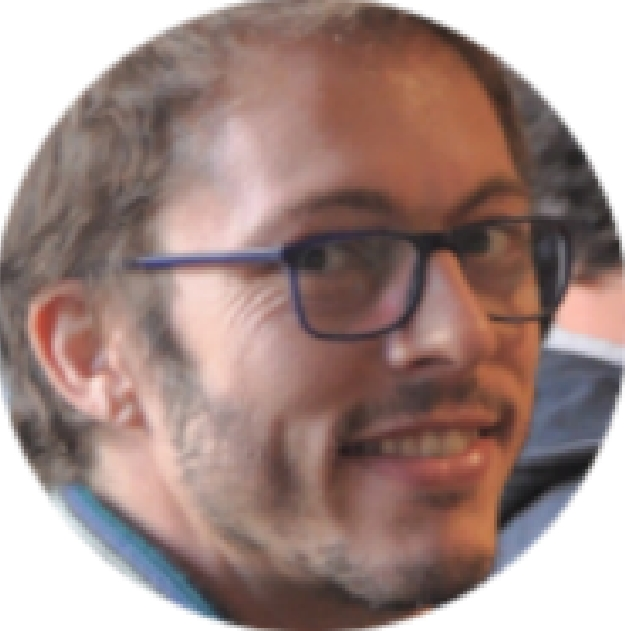
\includegraphics[width=\linewidth]{portrait.jpg}
        		\fcolorbox{white}{white}{\begin{minipage}[c][1.5cm][c]{1\mpwidth}
				\normalsize{ \textcolor{maincol} {Team Lead ``Transparent Social
Analytics''} }
			\end{minipage}}

		%---------------------------------------------------------------------------------------
		%	META SKILLS
		%----------------------------------------------------------------------------------------
				\icontext{caret-right}{12}{Konstanz, Germany}\\[6pt]
				\icontext{caret-right}{12}{german}\\[6pt]
				\icontext{caret-right}{12}{married}\\[6pt]
		
		
		\cvsection{Skills}

						\cvskill{R}{10+ yrs.}{1} \\[10pt]
								\cvskill{Python}{2 yrs.}{0.2} \\[10pt]
								\cvskill{JavaScript}{4 yrs.}{0.4} \\[10pt]
								\cvskill{Lua}{1 yr.}{0.1} \\[10pt]
								\cvskill{Rmarkdown}{6 yrs.}{0.6} \\[10pt]
								\cvskill{Quarto}{1 yr.}{0.1} \\[10pt]
								\cvskill{Data Analysis}{9 years}{0.9} \\[10pt]
								\cvskill{Web Scraping}{8 yrs.}{0.8} \\[10pt]
								\cvskill{Web Development}{8 years}{0.8} \\[10pt]
						
		\cvsection{Tools}

						\icontext{caret-right}{12}{Git}\\[6pt]
								\icontext{caret-right}{12}{RStudio}\\[6pt]
								\icontext{caret-right}{12}{VS Code}\\[6pt]
								\icontext{caret-right}{12}{Terminal}\\[6pt]
						
		\cvsection{Education}

						\cvmetaevent{09/2012 - 11/2015}{Ph.D.~Computer Science}{University of
Konstanz}{Thesis: Positional Approach for Network Centrality}
								\cvmetaevent{10/2006 - 07/2012}{Businessmathematics (Dipl.)}{Karlsruhe
Institute of Technology}{Thesis: Modularity Maximization}
						
		\cvsection{Contact}

						\icontext{map-marker}{16}{Konstanz, Germany}\\[6pt]
								\icontext{phone}{16}{+XX XXXX XXXX}\\[6pt]
								\icontext{envelope}{16}{david@schochastics.net}\\[6pt]
								\iconhref{home}{16}{mr.schochastics.net}{https://mr.schochastics.net}\\[6pt]
								\iconhref{github}{16}{schochastics}{https://github.com/schochastics}\\[6pt]
								\iconhref{twitter}{16}{schochastics}{https://twitter.com/schochastics}\\[6pt]
						
	\end{leftcolumn}

	\begin{rightcolumn}
		\cvsection{Summary} \vspace{4pt}

\cvtext{%
Lorem ipsum dolor sit amet, consetetur sadipscing elitr, sed diam nonumy
eirmod tempor invidunt ut labore et dolore magna aliquyam erat, sed diam
voluptua. At vero eos et accusam et justo duo dolores et ea rebum. Stet
clita kasd gubergren, no sea takimata sanctus est Lorem ipsum dolor sit
amet. Lorem ipsum dolor sit amet, consetetur sadipscing elitr, sed diam
nonumy eirmod tempor invidunt ut labore et dolore magna aliquyam erat,
sed diam voluptua. At vero eos et accusam et justo duo dolores et ea
rebum. Stet clita kasd gubergren, no sea takimata sanctus est Lorem
ipsum dolor sit amet.}

\cvsection{Experience} \vspace{4pt}

\cvevent{03/2022 - Present}{Team Lead for Transparent Social Analytics}{Department of Computational Social Science \newline GESIS - Leibniz Institute for the Social Sciences}{I am coordinating a project to build an Open Science platform with reusable code and tutorials to analyze digital behaviour data. I am also doing research on Open Science practices and I implement tools to enhance reproducibility and make methods accessible in R}

\cvevent{09/2018 - 02/2022}{Presidential Fellow}{Sociology Department \newline University of Manchester}{I did research on Disinformation on Social Media which involved the analysis of large scale and unstructured data sets with R and Bash}

\cvevent{11/2017 - 08/2018}{Post Doctoral Researcher}{Chair of Social Networks \newline ETH Zurich}{I developed new methods to analyze social networks and I gathered and analyzed large datsets from Social Media APIs}

\cvevent{10/2015 - 10/2017}{Post Doctoral Researcher}{Department of Computer \& Information Science \newline University of Konstanz}{I developed new methods to analyze social networks and scraped, harmonized, and analyzed a large corpus of football data}

\cvevent{11/2012 - 09/2015}{Ph.D. Candidate}{Department of Computer \& Information Science \newline University of Konstanz}{I developed new methods to analyze social networks and implemented these methods in R packages using R and C++}

\cvsection{Projects} \vspace{4pt}

\cvtext{%
See my \href{https://github.com/schochastics}{github profile} for a
comprehensive list of open source projects.}

\cvproj{R packages}{Creator and Maintainer}{edgebundle, graphlayouts, levelnet, netrankr, netUtils, networkdata, PSAWR, roughnet, roughsf, rtoot, Rtumblr, signnet, snahelper, webbotparseR, webtrackR}

\cvproj{R packages}{Contributor}{backbone, ggraph, multigraphr, netropy, rang, rgraph6}

\cvproj{Quarto extensions}{Creator and Maintainer}{Academicons (shortcodes), Blackboard (revealjs theme), sketchy (html theme), share buttons (filter), nutshell (filter), quartocities (website template), quartocv (cv templates)}

\cvproj{soccerverse.com (football analytics website)}{Creator and Maintainer}{Manual and automated gathering of football results around the world, Harmonizing data (e.g. club names and managers), Implementation of ranking algorithms, Predicting of league tables and matchforecasting, Uses R, JavaScript, HTML, and CSS, around 1000 visitors/month}
			\end{rightcolumn}
\end{paracol}


\end{document}
